%
% Chickens, Anyone?  (print folio)
% (c) 2009 Eric R. Jeschke (eric@redskieatnight.com).
% This work is licensed under a Creative Commons Attribution-Share Alike
% 3.0 United States License
% See http://creativecommons.org/licenses/by-sa/3.0/us/
%
% Eric Jeschke makes no representation about the suitability or accuracy
% of this software or data for any purpose, and makes no warranties,
% either express or implied, including merchantability and fitness for a
% particular purpose or that the use of this software or data will not
% infringe any third party patents, copyrights, trademarks, or other
% rights.  The software and data are provided "as is". 
%
% 
% If you make a .sty file, please let me know!
%
% [top-level file]
\nonstopmode

\documentclass[12pt,final]{article}
\usepackage{graphicx}
% where can I find the photos that will be imported for this version
\graphicspath{{./photos.web/}}

% Only uncomment if you have the fontspec package installed
% You will have to set the appropriate font names for what you have
% installed.
%
% You might be able to use opentype tools to find out the names of
% the fonts you can use here, or you can just experiment
%  $ otfinfo -a .../*.ttf
%
\usepackage{fontspec}
\setmainfont[Mapping=tex-text]{Garamond}
\setsansfont[Mapping=tex-text]{Arial}
\setmonofont[Mapping=tex-text]{Courier New}


% for setting the background
\usepackage[usenames]{color}

% in case you want to embed any hyperlinks
% turn on colorlinks to avoid the nasty box around the link
\usepackage[colorlinks=true,urlcolor=black]{hyperref}

% set this to printer paper size
\usepackage[paperwidth=11in, paperheight=8.5in, 
            left=1.5in, top=1.25in, right=1.5in, bottom=0.5in,
            nomarginpar,
            % center printed area on page
            vcentering, hcentering]{geometry}

% width of margin notes area
%\setlength{\marginparwidth}{0in}
% distance between margin and paragraph
%\setlength{\marginparsep}{0in}

% footer configuration 
\setlength{\footnotesep}{10pt}

% header configuration 
\setlength{\headheight}{10pt}
\setlength{\headsep}{0.1in}

\title{Chickens, Anyone?}
\author{Eric Jeschke}

%%%%%%%%% PDF/X-3 stuff, necessary for Blurb IF USING pdflatex %%%%%%%%%
%% \pdfinfo{
%% /Title (Chickens, Anyone?)   % set your title here
%% /Author (Eric Jeschke)       % set author name
%% /Subject (Chickens)          % set subject
%% /Keywords (Chickens, Hawaii) % set keywords
%% }
%% \pdfminorversion=4
%% \pdfcatalog{
%% /OutputIntents [ <<
%% /Info (none)
%% /Type /OutputIntent
%% /OutputConditionIdentifier (Web use)
%% /RegistryName (http://www.color.org/)
%% >> ]
%% }

%%%%%%%%% PDF stuff, IF USING xelatex %%%%%%%%%
\special{pdf:docinfo <<
/Title (Chickens, Anyone?)   % set your title here
/Author (Eric Jeschke)       % set author name
/Subject (Chickens)          % set subject
/Keywords (Chickens, Hawaii) % set keywords
  >>
}

% paragraph indentations
\setlength{\parindent}{0in}
% amount of space before each new paragraph begins
\setlength{\parskip}{1em}

% comment to force even justification
\raggedright

\begin{document}

\pagestyle{empty}
%\definecolor{photopagecol}{rgb}{0.65,0.65,0.65}
\definecolor{photopagecol}{rgb}{1.0,1.0,1.0}
\definecolor{textpagecol}{rgb}{1.0,1.0,1.0}
\pagecolor{textpagecol}

% define some useful commands for the photos

\newcommand{\signature}{\copyright \ Eric Jeschke}

\newcommand{\photo}[3][scale=1.0]{
{
  \includegraphics[#1]{#2}
  \begin{tabular*}{\textwidth}[t]{l@{\extracolsep{\fill}}r}
     \hspace*{0.5in} {\Large #3} & \signature \hspace*{0.5in} \\
  \end{tabular*}
}}

\newcommand{\kphoto}[3][scale=1.0]{
{
  \photo[#1]{#2}{#3}
  \renewcommand{\thefootnote}{}
  \footnote{#2}
}}

% bring in the rest of the content which is in common with the book
% version
%
% common information to the web version and print version
%
% images will be imported by searching the paths set with \graphicspath
% the book.tex or web.tex sets this so the correct resolution images end
% up in the correct document.
% 

% title page

{\huge This boy is from Steppe}
% front cover for web version
\includegraphics[width=4in]{me.jpg}

\begin{flushright}
{\Large by Lu Tao}
\end{flushright}
\newpage

% front matter page

\vspace*{1in}
{\LARGE About}
\vspace*{0.25in}

He's speed most of my childhood in Hohhot, Inner Mongolia. 
The scene of the steppe in my hometown keeps flashing back in his mind these days.  
And it inspires he to make this album in memory of my past days.
These photographs represent some part of him.
To some extent, to read this book is to read about this boy.

\vspace*{1.0in}

{\large Copyright \copyright \  2009 Eric R. Jeschke.  All Rights Reserved.}

This folio may not be reproduced in any form without written permission
of the author. 

{\tt eric@redskiesatnight.com}

\newpage

% here come the images, one per page
{ 
\pagecolor{photopagecol}

\kphoto[width=8in,height=6in]{R20090606-093158}{}
\newpage

\kphoto[width=8in]{R20090619-101312-curves}{}
\newpage

\kphoto[width=8in]{R20090619-101502-levels}{}
\newpage

\kphoto[width=8in]{R20090619-101707-curves}{}
\newpage

\kphoto[width=8in]{R20090619-101832-levels}{}
\newpage

\kphoto[width=8in]{R20090619-101948}{}
\newpage

\kphoto[width=8in]{R20090619-102238}{}
\newpage

\kphoto[width=8in]{R20090619-102446-curves}{}
\newpage

\kphoto[width=8in]{R20090619-102632-levels}{}
\newpage

\kphoto[width=8in]{R20090606-151823}{}
\newpage

\kphoto[width=8in]{R20090619-103748}{}
\newpage
}

\pagecolor{textpagecol}
\vspace*{1in}

{\LARGE Colophon}
\vspace*{0.25in}

Eric Jeschke finds life with a camera more fulfilling.
You can see more of Eric's photography at

\url{http://redskiesatnight.com/}

For more information about the book, {\em Chickens, Anyone?}, visit

\url{http://redskiesatnight.com/books/chickens-anyone}

\vspace*{0.25in}

This folio was created using \LaTeX and {\em xelatex}.
The font used is Garamond.

\vspace*{0.5in}

\begin{center}
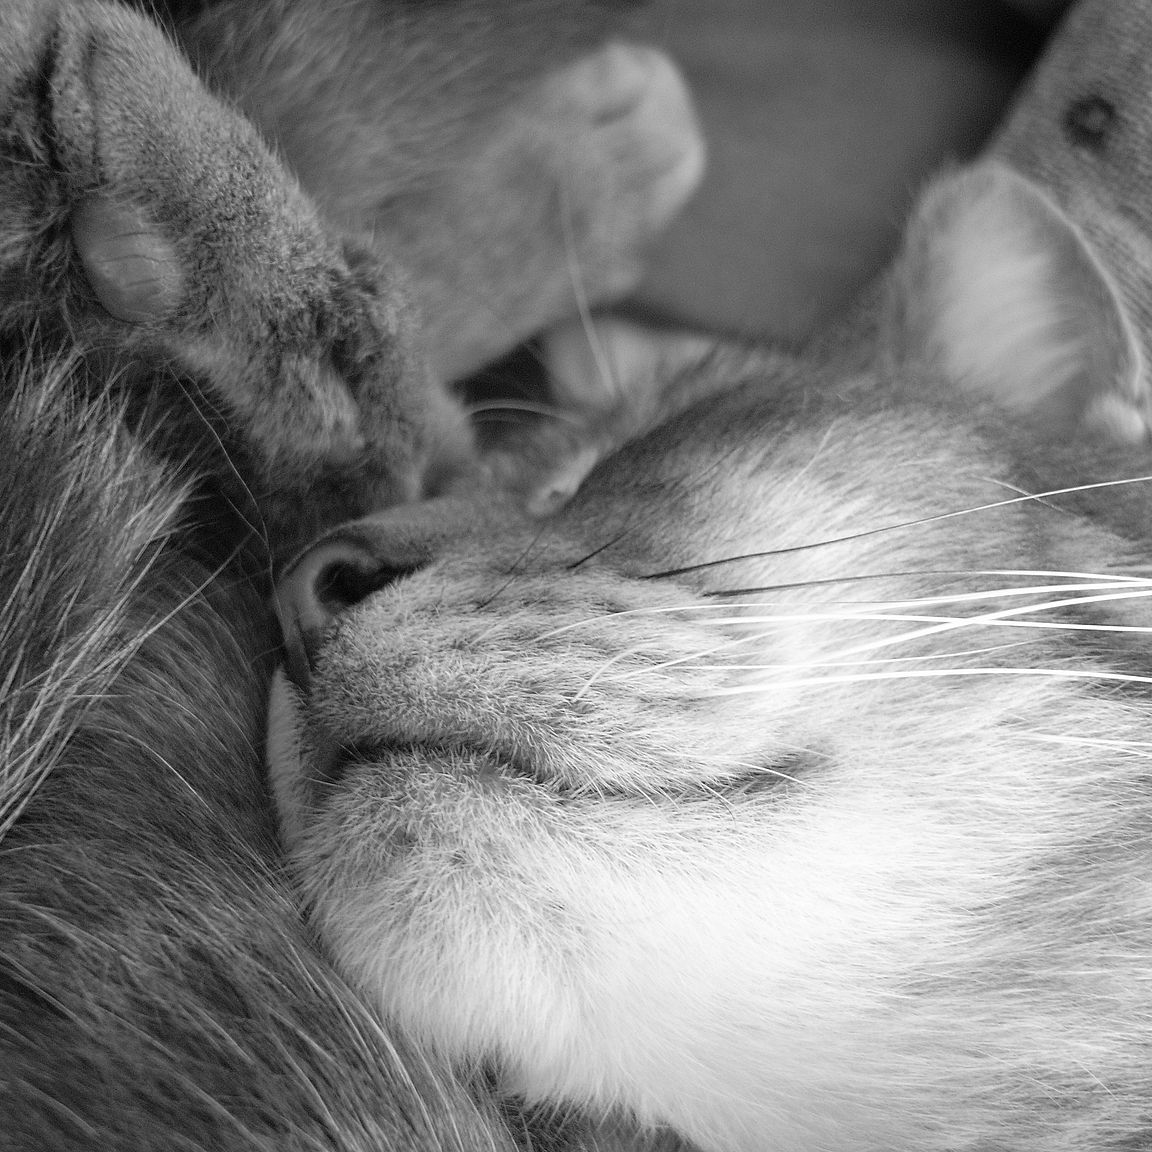
\includegraphics[width=1.5in]{R20080416-135900}
\end{center}

%END


\end{document}
